\documentclass{wticifes}

% ------------------------------------------------
% INÍCIO DO DOCUMENTO
% ------------------------------------------------
\begin{document}

% Espaçamento 1,5 para o texto principal
\onehalfspacing

\title{TÍTULO DO DOCUMENTO}
\maketitle
{Nome Autor 1}{Filiação Autor 1. \url{link lattes autor 1}. E-mail: \url{e-mail autor 1}}
{Nome Autor 2}{Filiação Autor 2. \url{link lattes autor 2}. E-mail: \url{e-mail autor 2}}
{Nome Autor 3}{Filiação Autor 3. \url{link lattes autor 3}. E-mail: \url{e-mail autor 3}}
% Para número diferente de autores (mais ou menos), editar
% o arquivo wticifes.cls, em todos os locais onde está
% indicado "TODO: automatizar"


\begin{resumo}
\lipsum[1]
\end{resumo}

\noindent\textbf{Palavras-chave:} key1, key2, key3

\vspace{0.5cm}
\begin{abstract}
\lipsum[1]
\end{abstract}

\noindent\textbf{Keywords:} key1, key2, key3

\section{Introdução}
Este é um modelo de documento que segue as especificações solicitadas. O texto está formatado com fonte tamanho 12, espaçamento entre linhas de 1,5 cm, sem espaçamento entre parágrafos. Exemplo de citação \cite{teste2023}.

Segundo \citeonline{fowler1997}.

\lipsum[1]

\section{Desenvolvimento}
As seções estão alinhadas à esquerda e sem numeração, conforme solicitado
nos requisitos.

\lipsum[1]

Abaixo segue um exemplo de citação longa, que deve ser formatada com recuo, espaçamento simples e fonte tamanho 10:

\begin{quote}
Esta é uma citação longa que deve ser formatada em espaço simples de entrelinhas e fonte tamanho 10. O texto está alinhado com recuo à esquerda para diferenciar do texto principal do documento, conforme as especificações solicitadas nos requisitos.
\end{quote}

\lipsum[3]

\begin{figure}
    \centering
    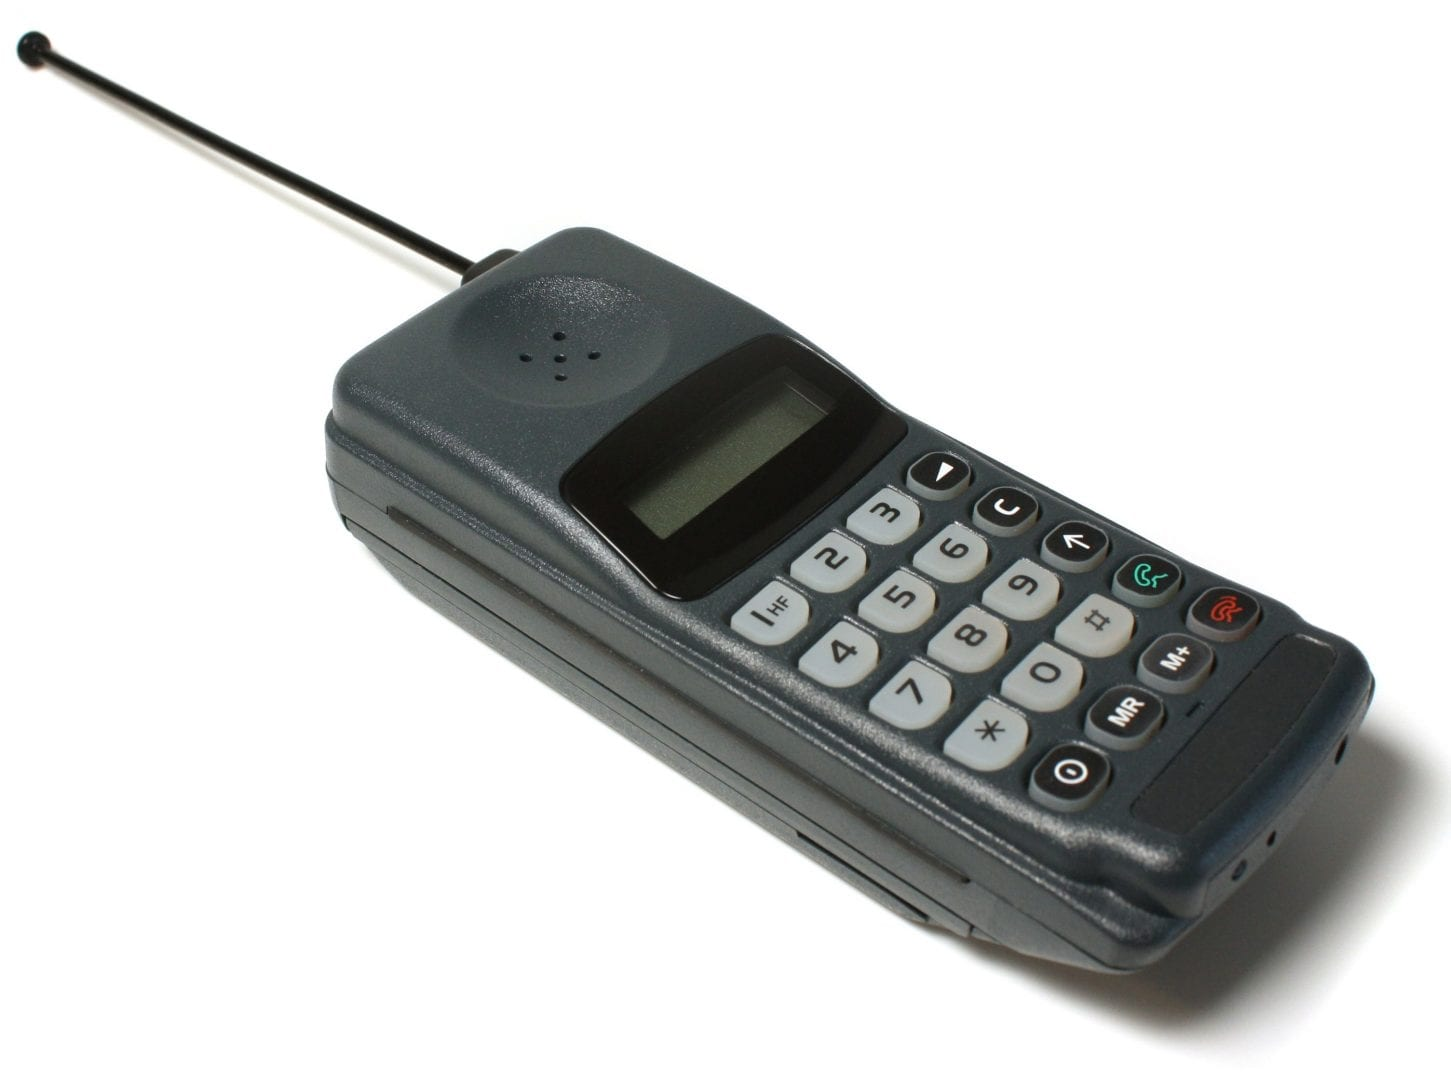
\includegraphics[width=0.5\linewidth]{img/img.jpg}
    \caption{Descrição}
    \label{fig:enter-label}
\end{figure}

\section{Considerações Finais}
\lipsum[2]

% Referências bibliográficas
\bibliographystyle{abntex2-alf}  % Estilo autor-data da ABNT
\bibliography{ref}  % Arquivo .bib contendo as referências


\end{document}